\chapter{Lecture \thechapter{} of 06/05/2026}

\section{Proximal mappings}

The topic is now the \emph{proximal mappings}, we will consider the book Convex Analysis by Dirk Lorentz and we will see proximal algorhitms and proximal mappings (chapter 8 + piece 10 + piece 12).

\begin{definition}[Proximal mapping/Monreau envelope]

    Let $f : \R^d \to \Rb$ proper convex closed, $\lambda \ge 0$. We define the \emph{proximal mapping} the map $\prox{\lambda f} : \R^d \to \R^d$ defined as 

    \[ \prox{\lambda f} (x) = \argmin_{y \in \R^d} \lambda f(y) + \frac12 \norm{y - x}^2. \]

    We can think it as a ''minimizer of the rescaled function $\lambda f$ + quadratic term''.

    We define the \emph{Monreau envelope} as 

    \[ M_{\lambda f} (x) = \inf_{y \in \R^d} f(y) + \frac{1}{2\lambda} \norm{y - x}^2. \]
    
\end{definition}

\begin{theorem}
    
    Let $f : \R^d \to \Rb$ be proper convex closed and fix $\lambda > 0$. The following holds:

    \begin{enumerate}
        \item for every $x \in \R^d$ there exists a unique $\hat{x}$ such that $\hat{x} = \prox{\lambda f} (x)$;
        \item $\hat{x}$ as above is characterized by the variational inequality 
            \[ \langle x - \hat{x} , y - \hat{x} \rangle + \lambda f(\hat{x}) - f(y) \le 0 \]
            for every $y \in \R^d$;
        \item $x^*$ is a minimizer of $f$ if and noly if $x^*$ is a fixed point of $\prox{\lambda f}$, i.e. $x^* = \prox{\lambda f}(x^*)$;
        \item the Monreau envelope $M_{\lambda f}$ is a convex differentiable function and $\nabla M_{\lambda f} = \frac{1}{\lambda} \left(x - \prox{\lambda f} (x) \right)$;
        \item it holds that 
            \[ \argmin_x f(x) = \argmin_x M_{\lambda f}(x). \]
    \end{enumerate}

\end{theorem}

\begin{proof}
    It's a bluff.
\end{proof}

\begin{example}
    
    Let $C$ be nonempt convex closed, $f(x) = \delta_C(x)$ the convex indicator function. Then 

    \begin{align*}
        \prox{\lambda f}(x) &= \argmin_{y \in \R^d} \lambda \delta_C(y) + \frac12 \norm{y-x}^2 \\
            &= \argmin_{y \in C} \frac12 \norm{y - x}^2  = P_C(x)
    \end{align*}

    the projection function of $C$. Moreover, 

    \begin{align*}
        M_{\lambda f} &= \frac{1}{2\lambda} \norm{P_C(x) - x}^2 \\
            &= \frac{1}{2\lambda} d(x,C)^2
    \end{align*}

    where $d(x,C) = \inf_{y \in C} \norm{x - y}$.

\end{example}

\begin{example}
    
    Let $f(x) = \abs{x}$, so $\hat{x} = \prox{\lambda f}(x) = \argmin_y \lambda \abs{y} + \frac12 (y-x)^2$. 

    Observe that if $x > 0$ then $\hat{x} > 0$ and $\prox{\lambda f}(-x) = - \prox[\lambda f](x)$, so we can compute only for $x \ge 0$, with $y \ge 0$. The minimum of the objective function is achived when its derivative is 0 (notice that the ''inside function'' is differentiable), hence $\lambda + y - x = 0 \implies y = x - \lambda$.

    All in all,

    \[ \prox{\lambda \abs{\cdot}}(x) = \begin{cases}
        x - \lambda \quad \text{if } x\ge\lambda \\
        0 \quad\text{if } - \lambda < x < \lambda \\
        x + \lambda \quad\text{if } x \le -\lambda
    \end{cases}
    = \max(\abs{x} - \lambda, 0)\mathrm{sgn}(x).
    \]

    The Monreau envelope is the 

    \[ M_{\lambda f}(x) = \begin{cases}
        \abs{x} - \frac{\lambda}{2} \quad \text{if } \abs{x} \ge \lambda \\
        \\
        \frac{1}{2\lambda}x^2 \quad\text{if } \abs{x} < \lambda
    \end{cases}
    \]

    which is called \emph{Huber function}, a differentiable appproximation of $\abs{\cdot}$.

    \begin{figure}[H]
        \centering
        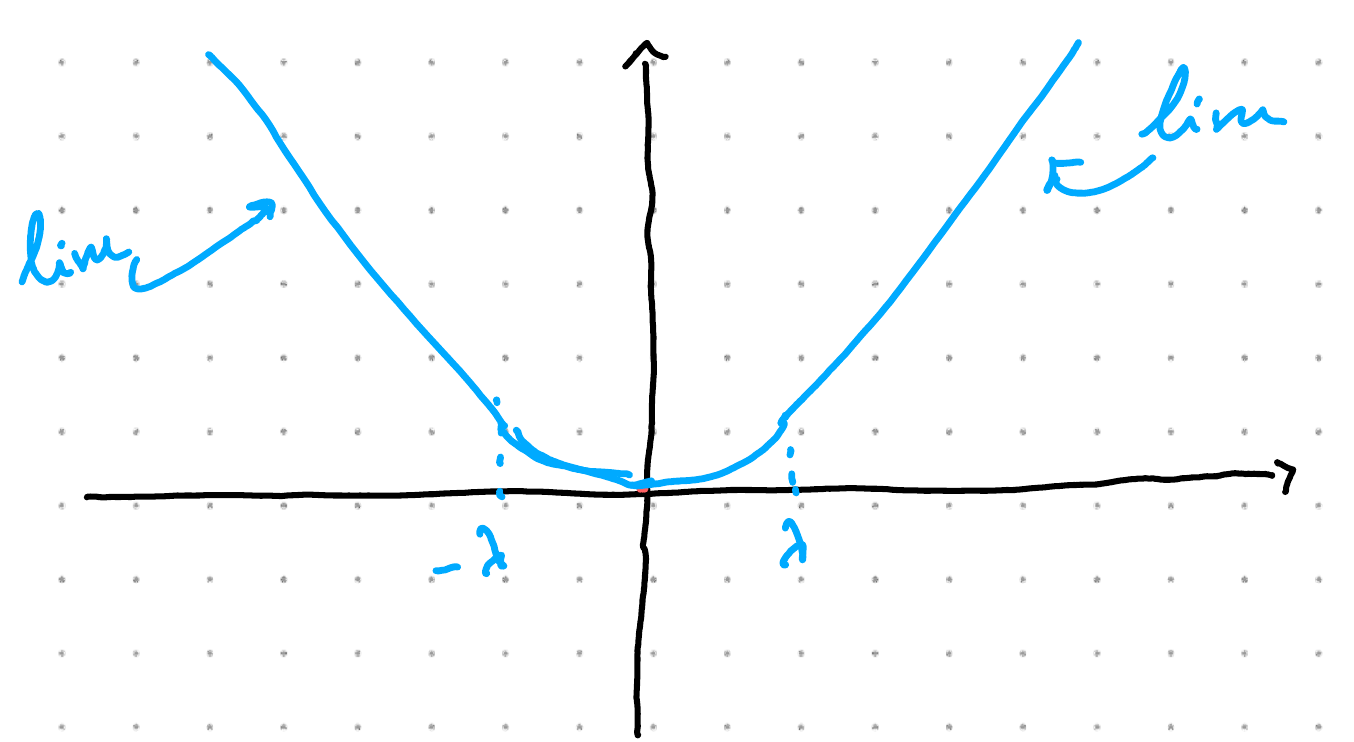
\includegraphics[width=0.7\textwidth]{img/mmodul.png}
        \caption{Monreau envelope of $\abs{\cdot}$ function}
    \end{figure}

\end{example}

\begin{proposition}
    
    \begin{enumerate}
        \item If $g(x) = \tau f(\mu x)$, $\tau, \mu \in \R$, $\tau > 0$ then 
            \[ \prox{\lambda g}(x) = \frac{1}{\mu} \prox{\lambda \mu^2 \tau f}(x); \]
        \item if $g(x) = f(Qx)$ with $Q$ orthonormal matrix, then
            \[ \prox{\lambda g}(x) = Q^\top \prox{\lambda f}(Qx). \] 
    \end{enumerate}

\end{proposition}

\subsection{Monreau identity}

\begin{theorem}[Monreau identity]

    Let $f : \R^d \to \Rb$ proper closed convex, $f^*(y) = \sup_x y^\top x - f(x)$. Then 

    \[ x = \prox{f} (x) + \prox{f^*}(x). \]
    
\end{theorem}

To prove this we need the following: 

\begin{lemma}
    
    Let $f,g : \R^d \to \Rb$ proper closed convex. Then if there exists $\bar{x} \in \dom{f} \cap \dom{g}$ with $f$ continous at $\bar{x}$ we have $\partial (f + g)(x) = \partial f(x) + \partial g(x)$.

\end{lemma}

\begin{proof}
    The proof is not difficoult but very technical and not short, uses Hahn-Banach, no further details.
\end{proof}

\begin{proof}(Monreau identity)

    Fix $\hat{x} = \prox{f}(x)$, then 

    \begin{align*}
        &0 \in \partial \left(f(\cdot) + \frac12 \norm{\cdot - x}^2\right)(\hat{x}) \\
        \implies &0 \in \partial f(\hat{x}) + \frac12 (\underbrace{\hat{x}-x}_{= \nabla \norm{\cdot}^2}) \\
        \implies &x - \hat{x} \in \partial f(\hat{x}).
    \end{align*}

    Recall that since $f$ is proper convex, then $f = f^{**}$. Let $y = x - \hat{x}$. Then $y \in \partial f(\hat{x}) \iff \hat{x} \in \partial f^*(y)$, hence 

    \begin{align*}
        &x-y \in \partial f^*(y) \\
        \implies &0 \in  \partial f^*(y) + (y-x) \\
        \implies &0 \in \partial \left(f^*(\cdot) + \frac12 \norm{\cdot - x}^2\right)(y)
    \end{align*}

    hence $y = \prox{f^*}(x)$. In the end, 

    \[ \prox{f}(x) + \prox{f^*}(x) = \hat{x} + y = \hat{x} + x - \hat{x} = x. \]
    
\end{proof}

In general $x = \prox{\lambda f}(x) + \prox{\frac{1}{\lambda} f^*}\left(\frac{x}{\lambda}\right)$.

